\section{Introduction}

Après le développement du moteur de détection des attaques SSH présenté dans le chapitre précédent ainsi que l'intégration des notifications automatiques via Telegram, l'étape suivante du projet consiste à mettre en œuvre un mécanisme de réponse automatique capable de neutraliser immédiatement une source d'attaque détectée.

L'objectif de cette phase est de connecter le système \textit{Automated Network Self-Defense System (ANSDS)} à un routeur Cisco IOS afin d'automatiser l'application de contre-mesures réseau. Contrairement à une approche reposant uniquement sur la génération d'alertes, le système développé est désormais capable d'agir directement sur l'infrastructure réseau en créant dynamiquement une liste de contrôle d'accès (\textit{Access Control List} -- ACL) destinée à bloquer l'adresse IP de l'attaquant.

Pour réaliser cette automatisation, la bibliothèque Python \textit{Netmiko} a été retenue. Cette bibliothèque permet d'établir des connexions SSH sécurisées avec des équipements réseau tout en simplifiant l'exécution de commandes Cisco IOS. Son intégration facilite le développement d'un module réutilisable capable d'administrer automatiquement le routeur sans intervention humaine.

Le développement a été réalisé de manière progressive afin de garantir la fiabilité de chaque composant. Les différentes étapes comprennent la préparation du routeur Cisco pour les connexions SSH, la validation des communications entre le serveur Ubuntu et le routeur, le développement du module Cisco, l'ajout d'une gestion robuste des exceptions, puis l'intégration complète avec le moteur de détection développé lors de la phase précédente.

À l'issue de cette phase, le système ANSDS est capable de détecter une attaque SSH, de transmettre une notification via Telegram, puis d'établir automatiquement une connexion SSH avec le routeur Cisco afin de créer une ACL bloquant immédiatement l'adresse IP malveillante.

Dans ce chapitre, nous présentons successivement les objectifs poursuivis, la préparation du routeur Cisco, l'installation et la configuration de Netmiko, le développement du module de réponse automatique, les mécanismes de gestion des exceptions, l'intégration avec le moteur de détection ainsi que les validations expérimentales réalisées.

\section{Objectifs de la phase}

Cette phase constitue la première étape du développement du mécanisme de réponse
automatique du projet ANSDS.

Les objectifs principaux sont les suivants :

\begin{itemize}

\item préparer le routeur Cisco afin d'accepter les connexions SSH sécurisées ;

\item valider la communication SSH entre le serveur Ubuntu et le routeur Cisco ;

\item installer et configurer la bibliothèque Python Netmiko ;

\item développer un premier script permettant d'établir une connexion distante avec le routeur ;

\item récupérer automatiquement les principales informations du routeur, notamment le nom d'hôte, la version du système Cisco IOS et les interfaces réseau ;

\item concevoir un module Cisco entièrement modulaire et réutilisable ;

\item développer une fonction capable de créer dynamiquement une liste de contrôle d'accès (ACL) afin de bloquer l'adresse IP d'un attaquant détecté ;

\item développer une fonction permettant de supprimer automatiquement cette ACL lorsque cela est nécessaire ;

\item protéger l'ensemble des opérations Netmiko à l'aide d'une gestion complète des exceptions afin d'assurer la robustesse du système en cas d'échec de connexion ou d'erreur d'authentification ;

\item intégrer le module Cisco au moteur de détection développé lors de la phase précédente afin d'automatiser entièrement la chaîne de détection et de réponse ;

\item valider expérimentalement le fonctionnement complet du système de réponse automatique.

\end{itemize}

À l'issue de cette phase, le système ANSDS est capable d'établir automatiquement une connexion SSH avec un routeur Cisco, d'y créer dynamiquement une ACL afin de bloquer une adresse IP malveillante détectée par Scapy, puis de poursuivre sa surveillance du trafic réseau sans interruption. Cette phase constitue une étape essentielle vers la mise en œuvre d'un système complet de détection et de réponse automatique aux attaques réseau.

\section{Préparation du routeur Cisco}

Avant de développer le mécanisme de réponse automatique, il a été nécessaire de préparer le routeur Cisco afin qu'il puisse accepter des connexions SSH provenant du serveur Ubuntu.

Cette étape constitue un prérequis indispensable au fonctionnement du module développé avec Netmiko. En effet, cette bibliothèque s'appuie sur le protocole SSH pour établir une connexion distante avec les équipements réseau et exécuter automatiquement des commandes Cisco IOS.

La préparation du routeur comprend la configuration du service SSH ainsi que la validation d'une première connexion distante depuis le serveur Ubuntu. Ces vérifications permettent de garantir que l'environnement est correctement configuré avant de commencer le développement du module de réponse automatique.

\subsection{Configuration SSH du routeur}

Le routeur Cisco a été configuré afin d'autoriser les connexions SSH sécurisées.

Cette configuration comprend notamment la définition du nom de domaine, la création d'un utilisateur local, la génération d'une paire de clés RSA ainsi que l'activation du protocole SSH version 2.

Ces paramètres permettent au routeur d'accepter des connexions d'administration distantes tout en bénéficiant des mécanismes de sécurité offerts par le protocole SSH.

La Figure~\ref{fig:manual_ssh_connection} présente une connexion SSH réussie entre le serveur Ubuntu et le routeur Cisco.

\begin{figure}[H]
    \centering
    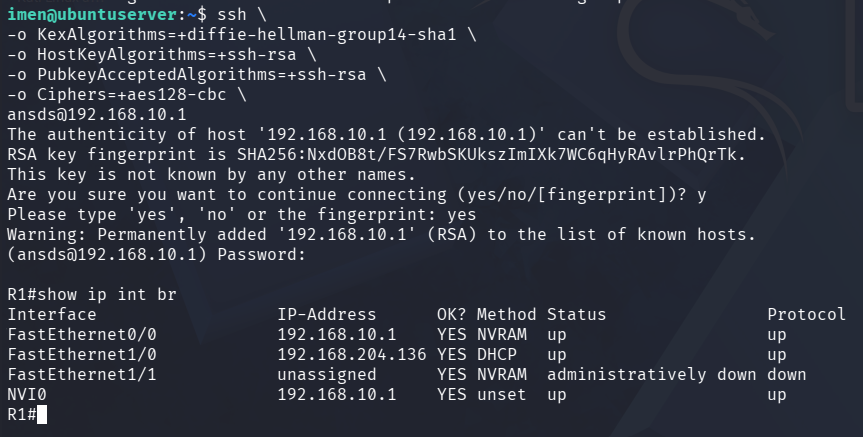
\includegraphics[width=\textwidth]{figures/Fig-04-01_Manual_SSH_Connection_To_Cisco.png}
    \caption{Connexion SSH manuelle entre le serveur Ubuntu et le routeur Cisco}
    \label{fig:manual_ssh_connection}
\end{figure}

\subsection{Validation de la connexion SSH}

Une fois la configuration terminée, une connexion SSH a été établie avec succès entre le serveur Ubuntu et le routeur Cisco.

Cette validation confirme le bon fonctionnement de la configuration SSH ainsi que la connectivité réseau entre les deux équipements.

Elle garantit également que le routeur est prêt à être administré automatiquement par le futur module Cisco développé avec Netmiko.

Cette étape est essentielle, car l'ensemble des opérations de réponse automatique réalisées dans les sections suivantes reposent sur cette connexion SSH.

\section{Installation et configuration de Netmiko}

Après avoir validé la communication SSH entre le serveur Ubuntu et le routeur Cisco, l'étape suivante consiste à intégrer une bibliothèque Python capable d'automatiser les interactions avec les équipements réseau.

Dans le cadre du projet ANSDS, la bibliothèque \textit{Netmiko} a été retenue en raison de sa simplicité d'utilisation et de sa compatibilité avec les équipements Cisco IOS. Cette bibliothèque permet d'établir des connexions SSH, d'exécuter des commandes de supervision ou de configuration et de récupérer automatiquement les informations retournées par le routeur.

Avant de développer le module de réponse automatique, plusieurs validations ont été réalisées afin de vérifier le bon fonctionnement de Netmiko ainsi que la communication entre Python et le routeur Cisco.

\subsection{Installation de la bibliothèque}

La bibliothèque Netmiko a été installée dans l'environnement virtuel Python utilisé durant le développement du projet.

L'utilisation d'un environnement virtuel permet d'isoler les dépendances logicielles du projet, de garantir la reproductibilité de l'environnement de développement et de faciliter son déploiement sur une autre machine.

Après l'installation, plusieurs vérifications ont été effectuées afin de confirmer que la bibliothèque était correctement installée et prête à être utilisée.

La Figure~\ref{fig:netmiko_installation} présente l'installation et la validation de Netmiko.

\begin{figure}[H]
    \centering
    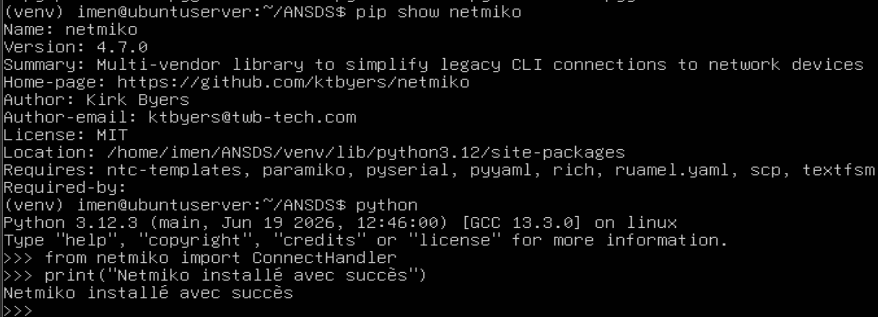
\includegraphics[width=\textwidth]{figures/Fig-04-02_Netmiko_Installation.png}
    \caption{Installation de la bibliothèque Netmiko}
    \label{fig:netmiko_installation}
\end{figure}

\subsection{Premier test de connexion}

Une fois Netmiko installé, un premier script de validation a été développé afin de vérifier la capacité de Python à établir une connexion SSH avec le routeur Cisco.

Ce script utilise la fonction \texttt{ConnectHandler()} de Netmiko afin d'ouvrir une session SSH en utilisant les paramètres de connexion du routeur. L'objectif de cette première expérimentation est de confirmer que les échanges entre le serveur Ubuntu et le routeur Cisco peuvent être automatisés sans intervention manuelle.

La réussite de cette connexion constitue une étape essentielle avant le développement des fonctions de configuration automatique qui seront intégrées au système ANSDS.

La Figure~\ref{fig:first_netmiko_connection} présente le résultat de cette première connexion.

\begin{figure}[H]
    \centering
    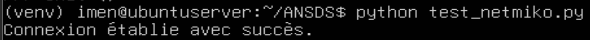
\includegraphics[width=\textwidth]{figures/Fig-04-03_First_Netmiko_Connection.png}
    \caption{Première connexion établie avec Netmiko}
    \label{fig:first_netmiko_connection}
\end{figure}

\subsection{Récupération automatique des informations du routeur}

Après la validation de la connexion SSH, le script de test a été enrichi afin de récupérer automatiquement plusieurs informations relatives au routeur Cisco.

Les commandes exécutées permettent notamment d'obtenir le nom d'hôte du routeur, la version du système Cisco IOS ainsi que la liste des interfaces réseau configurées.

Cette étape démontre que Netmiko ne se limite pas à l'établissement d'une connexion SSH, mais permet également d'automatiser l'exécution de commandes d'administration sur les équipements Cisco. Cette capacité constitue la base des futures opérations de configuration réalisées par le module de réponse automatique.

La Figure~\ref{fig:router_information_retrieval} présente les informations récupérées automatiquement.

\begin{figure}[H]
    \centering
    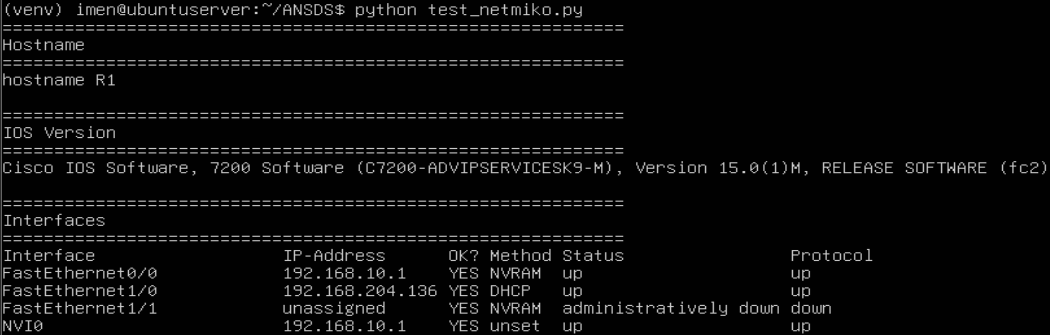
\includegraphics[width=\textwidth]{figures/Fig-04-04_Router_Information_Retrieval.png}
    \caption{Récupération automatique des informations du routeur Cisco}
    \label{fig:router_information_retrieval}
\end{figure}

\section{Développement du module Cisco}

Après la validation de la communication entre Python et le routeur Cisco, l'étape suivante consiste à développer un module dédié à la réponse automatique du système ANSDS.

Afin de garantir une architecture modulaire et facilement maintenable, toutes les fonctionnalités liées au routeur Cisco ont été regroupées dans un module indépendant nommé \texttt{cisco\_acl\_manager.py}. Cette approche permet de séparer les opérations de détection des opérations de réponse automatique tout en facilitant la réutilisation du code dans les phases suivantes du projet.

Le module développé est responsable de l'établissement de la connexion SSH avec le routeur Cisco, de l'exécution des commandes de configuration, de la création et de la suppression des listes de contrôle d'accès (ACL), ainsi que de la gestion des erreurs pouvant survenir lors des communications avec l'équipement réseau.

\subsection{Architecture modulaire}

Le projet ANSDS repose sur une architecture modulaire dans laquelle chaque composant possède une responsabilité bien définie.

Le moteur de détection développé avec Scapy est chargé d'observer le trafic réseau et d'identifier les comportements suspects. Le module Telegram assure l'envoi des notifications tandis que le module Cisco est responsable de la réponse automatique sur l'infrastructure réseau.

Cette séparation des responsabilités améliore la lisibilité du code, facilite les opérations de maintenance et permet de faire évoluer indépendamment chacun des modules du système.

\subsection{Création du module \texttt{cisco\_acl\_manager.py}}

Le module \texttt{cisco\_acl\_manager.py} constitue le cœur du mécanisme de réponse automatique développé durant cette phase.

Ce module centralise l'ensemble des opérations réalisées sur le routeur Cisco. Il établit une connexion SSH sécurisée à l'aide de Netmiko, exécute les commandes de configuration Cisco IOS puis ferme automatiquement la connexion une fois les opérations terminées.

Afin de renforcer la sécurité du projet, les paramètres de connexion du routeur (adresse IP, nom d'utilisateur et mot de passe) sont stockés dans un fichier \texttt{.env}. Cette approche évite l'exposition d'informations sensibles dans le code source tout en facilitant le déploiement du projet sur différents environnements.

\subsection{Création dynamique d'une ACL}

Une fonction nommée \texttt{block\_ip()} a été développée afin de créer automatiquement une liste de contrôle d'accès sur le routeur Cisco.

Cette fonction reçoit en paramètre l'adresse IP source détectée par le moteur Scapy. Elle construit ensuite les commandes Cisco IOS nécessaires à la création d'une règle de filtrage bloquant immédiatement tout trafic provenant de cette adresse.

La règle générée adopte le format suivant :

\begin{center}
\texttt{deny ip host <SOURCE\_IP> any}
\end{center}

Cette approche permet de transformer automatiquement une détection d'attaque en une action de protection sans intervention de l'administrateur.

La Figure~\ref{fig:dynamic_acl_creation} présente la création dynamique de l'ACL sur le routeur Cisco.

\begin{figure}[H]
    \centering
    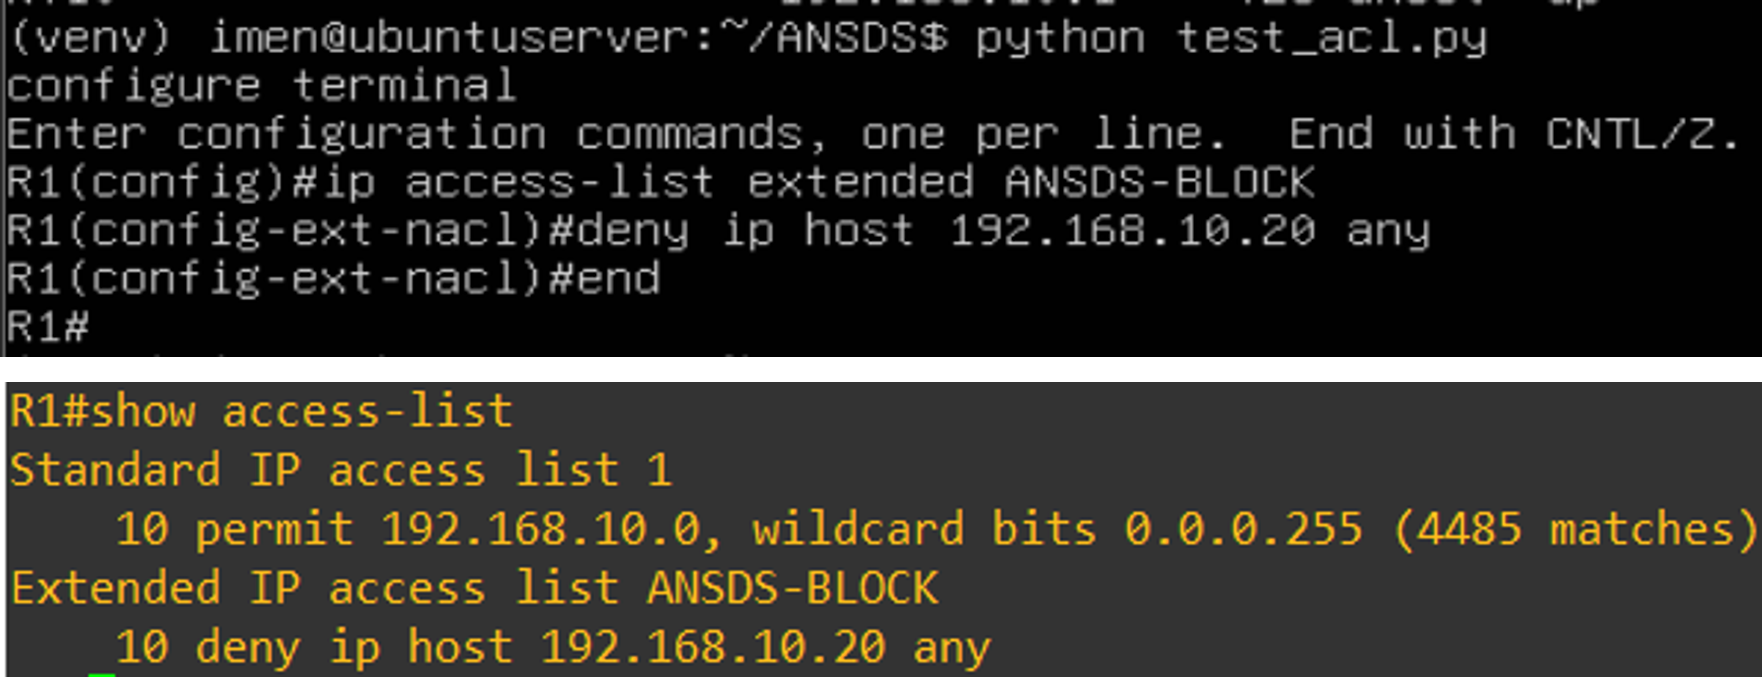
\includegraphics[width=\textwidth]{figures/Fig-04-05_Dynamic_ACL_Creation.png}
    \caption{Création dynamique d'une ACL avec Netmiko}
    \label{fig:dynamic_acl_creation}
\end{figure}

\subsection{Suppression automatique d'une ACL}

Une seconde fonction, nommée \texttt{remove\_acl()}, a été développée afin de supprimer automatiquement la liste de contrôle d'accès créée précédemment.

Cette fonctionnalité permet de rétablir rapidement l'état initial du routeur après les phases de validation ou lorsqu'une règle de filtrage n'est plus nécessaire.

La suppression automatique des ACL facilite les campagnes de tests successives et améliore la réutilisabilité du système sans nécessiter de reconfiguration manuelle du routeur.

La Figure~\ref{fig:dynamic_acl_removal} présente la suppression de l'ACL créée durant les expérimentations.

\begin{figure}[H]
    \centering
    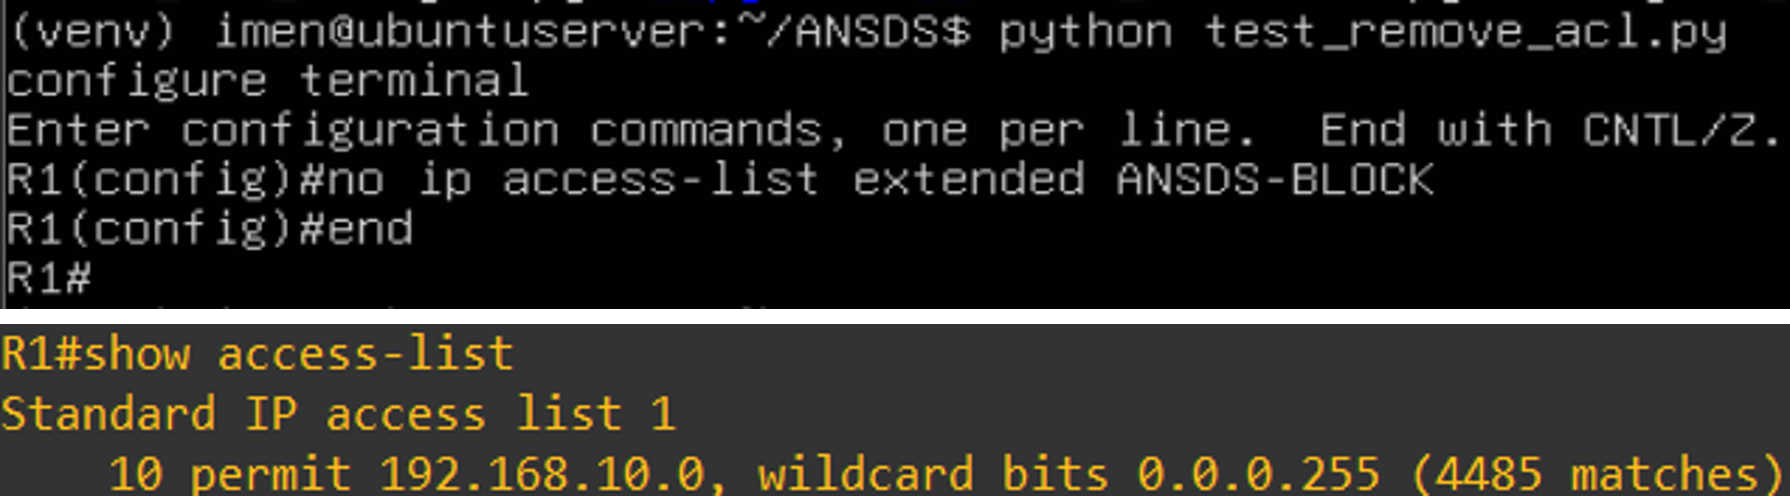
\includegraphics[width=\textwidth]{figures/Fig-04-06_Dynamic_ACL_Removal.png}
    \caption{Suppression automatique d'une ACL}
    \label{fig:dynamic_acl_removal}
\end{figure}

\section{Gestion des exceptions}

Dans un système de réponse automatique, la fiabilité des communications avec les équipements réseau constitue un élément essentiel. Une interruption de la connexion SSH, une erreur d'authentification ou tout autre incident ne doivent pas provoquer l'arrêt du système ANSDS.

Afin d'assurer la robustesse du module Cisco, toutes les opérations réalisées avec Netmiko ont été protégées à l'aide d'une gestion complète des exceptions (\texttt{try/except/finally}).

Cette approche permet d'intercepter les erreurs susceptibles de survenir lors de l'établissement de la connexion SSH ou de l'exécution des commandes Cisco IOS, tout en garantissant la poursuite du fonctionnement du moteur de détection.

\subsection{Gestion des erreurs de communication}

Le module Cisco intercepte les principales exceptions pouvant être générées par Netmiko.

Une première exception, \texttt{NetmikoTimeoutException}, est déclenchée lorsque le routeur Cisco ne répond pas dans le délai prévu ou devient momentanément indisponible.

Une seconde exception, \texttt{NetmikoAuthenticationException}, est levée lorsque les informations d'authentification utilisées pour établir la connexion SSH sont incorrectes.

Dans ces deux situations, le module affiche un message explicite permettant d'identifier rapidement l'origine du problème tout en évitant l'arrêt brutal de l'application.

\subsection{Utilisation des blocs \texttt{try}, \texttt{except} et \texttt{finally}}

Toutes les opérations de configuration réalisées par le module Cisco sont encapsulées dans un bloc \texttt{try}.

Les différents blocs \texttt{except} permettent de traiter séparément les erreurs de communication, les erreurs d'authentification ainsi que toute autre exception inattendue pouvant survenir durant l'exécution du programme.

Enfin, le bloc \texttt{finally} garantit la fermeture systématique de la connexion SSH avec le routeur Cisco, indépendamment du résultat des opérations réalisées.

Cette approche permet de libérer correctement les ressources réseau et d'éviter qu'une connexion reste ouverte en cas d'erreur.

\subsection{Validation du mécanisme de gestion des exceptions}

Le bon fonctionnement de la gestion des exceptions a été validé en provoquant volontairement une erreur d'authentification lors de l'établissement de la connexion SSH avec le routeur Cisco.

Le système intercepte correctement l'exception générée par Netmiko, affiche un message d'erreur explicite puis termine proprement son exécution sans provoquer l'arrêt du programme.

Cette validation confirme la robustesse du module Cisco et garantit que le système ANSDS pourra continuer à fonctionner même en présence d'un problème temporaire de communication avec le routeur.

La Figure~\ref{fig:netmiko_exception_handling} présente le résultat de cette validation.

\begin{figure}[H]
    \centering
    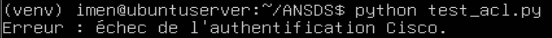
\includegraphics[width=\textwidth]{figures/Fig-04-07_Netmiko_Exception_Handling_Authentication_Error.png}
    \caption{Validation de la gestion des exceptions Netmiko}
    \label{fig:netmiko_exception_handling}
\end{figure}

\section{Intégration avec le moteur de détection}

Après avoir développé et validé indépendamment le moteur de détection SSH, le module de notification Telegram ainsi que le module Cisco, l'étape suivante consiste à intégrer l'ensemble de ces composants au sein d'une architecture unique de réponse automatique.

L'objectif de cette intégration est de permettre au système ANSDS d'enchaîner automatiquement les différentes opérations depuis la détection d'une attaque jusqu'à l'application d'une contre-mesure sur le routeur Cisco, sans intervention humaine.

Cette approche transforme le système développé en une véritable plateforme automatisée de détection et de réponse aux incidents de sécurité.

\subsection{Transmission de l'adresse IP détectée}

Le moteur de détection développé avec Scapy surveille en permanence le trafic SSH circulant sur le réseau.

Lorsqu'une adresse IP dépasse le seuil de tentatives de connexion défini, le détecteur identifie cette adresse comme potentiellement malveillante.

Cette adresse IP est ensuite transmise directement au module Cisco en appelant la fonction \texttt{block\_ip(ip\_src)}.

L'utilisation d'un paramètre permet au module Cisco de rester totalement indépendant du moteur de détection. Ainsi, la même fonction peut être réutilisée ultérieurement avec d'autres mécanismes de détection sans nécessiter de modification du code.

\subsection{Enchaînement automatique des modules}

Une fois le seuil de détection atteint, le système exécute automatiquement les différentes opérations selon une séquence prédéfinie.

Le moteur Scapy détecte tout d'abord l'activité suspecte et construit le message d'alerte contenant les principales informations relatives à l'attaque.

Ce message est ensuite transmis au module Telegram afin d'informer l'administrateur du réseau.

Après l'envoi de cette notification, le module Cisco établit automatiquement une connexion SSH avec le routeur Cisco à l'aide de Netmiko puis crée dynamiquement une ACL permettant de bloquer immédiatement l'adresse IP détectée.

Cette séquence assure une transition entièrement automatique entre la phase de détection et la phase de réponse, réduisant ainsi considérablement le temps de réaction face à une attaque.

\subsection{Architecture finale du système}

À l'issue de cette phase, les différents modules développés depuis le début du projet fonctionnent de manière coordonnée afin de constituer une chaîne complète de détection et de réponse automatique.

L'architecture finale du système peut être résumée selon la séquence suivante :

\begin{center}

Attaquant

$\downarrow$

Scapy

$\downarrow$

Détection SSH

$\downarrow$

Notification Telegram

$\downarrow$

Netmiko

$\downarrow$

Routeur Cisco

$\downarrow$

ACL dynamique

$\downarrow$

Blocage automatique de l'adresse IP

\end{center}

Cette architecture modulaire facilite les évolutions futures du projet. Chaque composant peut être amélioré indépendamment tout en conservant une interface claire avec les autres modules du système.

\section{Validation expérimentale}

Après le développement et l'intégration du module Cisco, plusieurs expérimentations ont été réalisées afin de valider progressivement chacune des fonctionnalités développées.

Chaque validation a été effectuée de manière indépendante avant de vérifier le fonctionnement complet de la chaîne de détection et de réponse automatique.

Les expérimentations portent successivement sur la communication avec le routeur Cisco, la création dynamique des ACL, leur suppression, la robustesse du module face aux erreurs de communication ainsi que l'intégration complète avec le moteur de détection développé dans le chapitre précédent.

\subsection{Validation de la communication avec le routeur Cisco}

La première série d'expérimentations consiste à vérifier que le module Netmiko est capable d'établir une connexion SSH avec le routeur Cisco puis d'exécuter automatiquement plusieurs commandes d'administration.

Les résultats obtenus montrent que le système récupère correctement le nom d'hôte du routeur, la version du système Cisco IOS ainsi que les informations relatives aux interfaces réseau.

Cette validation confirme que le module développé peut administrer automatiquement le routeur Cisco et constitue une base fiable pour les opérations de réponse automatique.

La Figure~\ref{fig:router_information_retrieval} illustre les informations récupérées automatiquement lors de cette expérimentation.

\subsection{Validation de la création dynamique d'une ACL}

Une seconde expérimentation a été réalisée afin de vérifier le bon fonctionnement de la fonction \texttt{block\_ip()}.

Lors de cette validation, le module Cisco établit automatiquement une connexion SSH avec le routeur puis crée une liste de contrôle d'accès nommée \texttt{ANSDS-BLOCK}.

L'adresse IP transmise au module est immédiatement intégrée dans une règle de filtrage Cisco IOS, ce qui permet de bloquer automatiquement tout trafic provenant de cette source.

La présence de cette ACL a ensuite été vérifiée directement sur le routeur à l'aide des commandes d'administration Cisco.

La Figure~\ref{fig:dynamic_acl_creation} présente le résultat obtenu.

\subsection{Validation de la suppression automatique d'une ACL}

Afin de compléter le mécanisme de réponse automatique, une expérimentation supplémentaire a été réalisée pour valider le fonctionnement de la fonction \texttt{remove\_acl()}.

Cette fonction supprime automatiquement la liste de contrôle d'accès précédemment créée sur le routeur Cisco.

La vérification de la configuration du routeur confirme que l'ACL est correctement supprimée, ce qui permet de retrouver l'état initial du système avant une nouvelle campagne de tests.

La Figure~\ref{fig:dynamic_acl_removal} présente le résultat de cette validation.

\subsection{Validation de la robustesse du module Cisco}

Le fonctionnement du mécanisme de gestion des exceptions a également été validé.

Pour cette expérimentation, une erreur d'authentification a volontairement été provoquée afin de vérifier la réaction du système.

Les résultats montrent que le module intercepte correctement l'exception générée par Netmiko, affiche un message d'erreur explicite puis termine proprement son exécution sans provoquer l'arrêt de l'application.

Cette validation confirme que le système ANSDS reste opérationnel même lorsqu'une erreur survient durant la communication avec le routeur Cisco.

La Figure~\ref{fig:netmiko_exception_handling} présente cette expérimentation.

\subsection{Validation de la chaîne complète de détection et de réponse}

La dernière expérimentation consiste à valider le fonctionnement complet du système ANSDS après l'intégration du module Cisco.

Une série de tentatives de connexion SSH est générée depuis la machine Kali Linux afin de dépasser le seuil de détection configuré dans le moteur Scapy.

Lorsque ce seuil est atteint, le système détecte automatiquement l'activité suspecte, construit une notification contenant les principales informations relatives à l'attaque puis transmet cette notification via Telegram.

Après l'envoi de cette alerte, le module Cisco établit automatiquement une connexion SSH avec le routeur et crée une ACL permettant de bloquer immédiatement l'adresse IP de l'attaquant.

Les résultats obtenus démontrent le bon fonctionnement de l'ensemble de la chaîne de traitement développée durant les différentes phases du projet.

La Figure~\ref{fig:complete_detection_response} présente cette validation finale.

\begin{figure}[H]
    \centering
    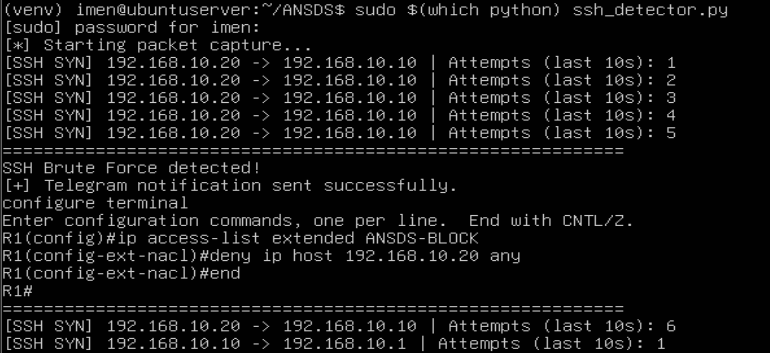
\includegraphics[width=\textwidth]{figures/Fig-04-08_Complete_Automated_Detection_And_Response.png}
    \caption{Validation complète de la chaîne de détection et de réponse automatique}
    \label{fig:complete_detection_response}
\end{figure}

\section{Analyse des résultats}

Les différentes expérimentations réalisées au cours de cette phase montrent que l'ensemble des objectifs fixés a été atteint.

La préparation du routeur Cisco et la validation des communications SSH ont permis d'établir une infrastructure fiable pour les opérations d'administration automatique. L'utilisation de la bibliothèque Netmiko a ensuite facilité le développement d'un module capable d'exécuter automatiquement des commandes Cisco IOS depuis le serveur Ubuntu.

Le module \texttt{cisco\_acl\_manager.py} développé durant cette phase assure la création et la suppression dynamiques des listes de contrôle d'accès tout en conservant une architecture modulaire et facilement réutilisable. La séparation entre les fonctions de détection, de notification et de réponse améliore la lisibilité du code et simplifie les futures évolutions du projet.

Les mécanismes de gestion des exceptions intégrés au module Cisco renforcent également la robustesse du système. Les différentes expérimentations ont montré que les erreurs de communication ou d'authentification sont correctement prises en charge sans provoquer l'arrêt du moteur de détection.

Enfin, l'intégration du module Cisco avec le moteur Scapy et le module Telegram permet désormais d'obtenir une chaîne complète de détection et de réponse automatique. Dès qu'une activité suspecte est détectée, le système génère une alerte, informe l'administrateur puis applique immédiatement une contre-mesure sur le routeur Cisco en créant dynamiquement une ACL de blocage.

Les résultats obtenus démontrent que l'architecture développée répond aux objectifs fixés pour cette phase et constitue une base solide pour les prochaines évolutions du projet ANSDS.

\section{Conclusion}

Au cours de cette quatrième phase, le système ANSDS a été enrichi d'un mécanisme de réponse automatique reposant sur l'administration d'un routeur Cisco à l'aide de la bibliothèque Netmiko.

Les différentes expérimentations ont permis de valider la préparation du routeur pour les connexions SSH, l'installation et la configuration de Netmiko, le développement d'un module Cisco modulaire, la création et la suppression automatiques d'une liste de contrôle d'accès ainsi que la gestion robuste des exceptions.

L'intégration de ce module avec le moteur de détection développé précédemment permet désormais au système d'assurer automatiquement l'ensemble de la chaîne de traitement, depuis la détection d'une attaque SSH jusqu'au blocage immédiat de l'adresse IP malveillante sur le routeur Cisco.

Cette évolution constitue une étape importante dans la réalisation du projet ANSDS puisqu'elle transforme le système en une plateforme capable non seulement de détecter les activités suspectes mais également de réagir automatiquement afin de limiter leur impact sur le réseau.

La phase suivante sera consacrée à l'amélioration du système de réponse automatique et à l'ajout de nouvelles fonctionnalités permettant d'accroître la sécurité, la flexibilité et les capacités d'administration de l'architecture développée.